%\documentclass[10pt][runningheads]{llncs}
\documentclass[10pt]{llncs}
%\documentclass[transaction]{IEEEtran}
% IEEETran already defines natbib package. undefined it so that we can use a more customized natbib
\makeatletter
\let\NAT@parse\undefined
\makeatother
%% INFOCOM 2010 addition: 
\makeatletter
\def\ps@headings{%
\def\@oddhead{\mbox{}\scriptsize\rightmark \hfil \thepage}%
\def\@evenhead{\scriptsize\thepage \hfil \leftmark\mbox{}}%
\def\@oddfoot{}%
\def\@evenfoot{}}
\makeatother
%\pagestyle{headings}
%Furthermore change the line \pagestyle{headings} to \pagestyle{empty}
\usepackage{float}
\usepackage[pdftex]{graphicx}
\usepackage{upgreek}
%\usepackage[hang,tight]{subfigure}
\usepackage{subfigure}
\usepackage{subfloat}
%\usepackage{algorithm2e}
%\usepackage[ruled,algonl]{algorithm2e}
\usepackage[ruled,vlined,resetcount,algochapter]{algorithm2e}
\usepackage{epsfig}
\usepackage{fullpage}
\usepackage{setspace}
\usepackage{verbatim}
\usepackage{amsfonts}
\usepackage{tabularx}
%\usepackage[sorting=none]{biblatex}
\usepackage[square, comma, sort, numbers]{natbib}
%\usepackage[round]{natbib}   % omit 'round' option if you prefer square brackets
\usepackage{amsmath}
\usepackage{booktabs}
\usepackage{enumerate}
%\usepackage{url}
%
%============================================================
\makeatletter
\renewcommand\bibsection%
{
  \section*{\refname
    \@mkboth{\MakeUppercase{\refname}}{\MakeUppercase{\refname}}}
}
\makeatother
%============================================================
\newenvironment{algorithmfloating}{%
\renewenvironment{algocf}[1][h]{}{}% pass over the floating stuff
\algorithm
}{%
\endalgorithm
}
%============================================================
%
%\doublespacing
%\setlength{\parskip}{12pt} % 12 pt = space between paragraphs
%\setlength{\parindent}{3pt} % 0 pt = indentation
\begin{document}
%\pagestyle{headings}
%\pagestyle{empty}
%
%============================================================
\title{Research Proposal: An interaction index based Deep Learning Framework for predictive and preventive measures for IoTs}
%
%============================================================
\author{
Nomica Choudhry (\selectfont\ttfamily\upshape nomica19@yahoo.com)\\
}

%abbreviated author list (for running head)
\authorrunning{Nomica Choudhry et. al.}

\institute{
Faculty of Science, Engineering and Built Environment, Deakins University\\
}
\maketitle

%
%==========================
\section{Introduction}
International Organization for Migration (Bret 2015) estimated that around 3 million people are moving to cities every week and by 2040 it is estimated that around 65\% population will be living in cities for better life style. Managing such a massive population and infrastructre with the intervention of technology is an interesting area of research and governments at different levels - regional, national, and international have initiated programs on digital and smart cities.

To make the concept of smart city a reality, Internet of Things (IoT) has gained significance attention (Vlacheas et al.). IoT is a network where wired and wireless devices; such as RFID (radio-frequency identification) systems, embedded sensors and actuator nodes, are inter-connected and communicate with each enabling smart and autonomous services. These services help solve the problems related to traffic management, climate change, urban planning, security and surveillance – to name a few. 

%
%----------------------------------------------------
\subsection{Background}
These IOT services utilize cloud based protocols and technologies to accumulate data from wireless and wired sensing devices. As this data is coming from different sources we need to pay attention to data breach cases and privacy threats. Security can esaily be compromised in IoT computing there are number of devices connected via different gateways. Each device has a different IP address, and any hacker can fake the IP address to gain access to the personal information that is stored in that particular IoT device.

Authentication, being an important issue of IoT computing, can not be ignored. A rouge IoT device is a device which passes oneself of as legal and persuade end user to connect to it. Once connected, it manipulates the signals coming to and from the user to the cloud and can easily launch attacks. Moreover, as IoT computing is based on wireless technology, privacy of the data is also a genuine problem. 

Nevertheless, due to the very large scale of the data sensed by the IoT devices, the security of the data accumulated with human intervention is not feasible. We need this sensed data to be secured an autonomous and self-sustained manner using artificial intelligence techniques. Machine learning and deep learning are two of the important artificial intelligence techniques used to identify security threats for IoT computing.

%
% ----------
% General Security Protocols for Fog Computing

%
% ----------
% AI based Security Protocols for Fog Computing


%
% ----------
% NN based Security Protocols for Fog Computing


%
% ----------
% Deep Learning based Security Protocols for Fog Computing


% Cons of the deep learning techniques
% NN with many layers pass input data through more mathematical operations than NN with few layers, and are therefore more computationally intensive to train. Computational intensivity is one of the hallmarks of deep learning NN, and it is one reason why a new kind of chip call GPUs are in demand to train deep-learning models.

%
%----------------------------------------------------
\subsection{Research Issues}


%
% ----------
% Research Issue # 1 in Deep Learning based Security Protocols for Fog Computing


%
% ----------
% Research Issue # 2 in Deep Learning based Security Protocols for Fog Computing


%
% ----------
% Research Issue # 3 in Deep Learning based Security Protocols for Fog Computing


%
%----------------------------------------------------
\subsection{Research Problem, Motivation and Objectives}

%
% ----------
\subsubsection{Research Probem}

% Explain the research problem we are addressing

%
% ----------
\subsubsection{Motivation}

% Expalin Why we are addressing this research problem

%
% ----------
% Why are we researching a security protocol?

%
% ----------
% Why are we researching an Deep Learning based security protocol?

%
% ----------
% Why are we researching a regression protocol?

%
% ----------
\subsubsection{Applications}
Recently, the adoption of fog and IoT in the healthcare field has been significantly improved health services and contributed to its innovation. Health monitoring systems have been using remote cloud servers for storing and processing huge amount of data coming from large amount of sensors. These systems however suffer from a lot of issues related to latency, location awareness and redundant data. These issues can not be tolerated in healthcare system as single error in analyzing data causes inaccurate treatment decisions and can cause precious human life. A better solution is to provide an extra layer in between a conventional gateway and a remote cloud server. The extra layer denoted as fog layer helps diminishing the volume of transmitted data for guaranteeing. QoS, and saving network bandwidth by preprocessing data. At the same times, fog computing offers advanced services at the edge of the network and reduces the burden of cloud.

%
% ----------
\subsubsection{Research Objective}

% Explain the purpose of this research and the objectives of this study


%
%----------------------------------------------------
\subsection{The Contributions}


%
%----------------------------------------------------
\subsection{Thesis Organization}


%
%==========================
\section{Survey}

% Overview of the Research in the field and Taxonomy

%
%----------------------------------------------------
\subsection{Neural Networks}
% What is a NN / ML?
Neural network based machine learning techniques are dynamic and do not require human intervention to make certain changes. This ability of neural network to modify itself when exposed to more data sets it apart from traditional artificial based security solutions, e.g. the knowledge graphs and expert systems. 

% What is importance of NN?
Neural networks are capable of discovering latent structures within unlabeled, unstructured data, which is the vast majority of data in the world.

% How does a typical NN work?
In short, all neural network based techniques are an optimization algorithm. They minimize their error by recursively keep on measuring the error and modifying their parameters until they can’t achieve any less error. Our goal in using a neural net is to arrive at the point of least error as fast as possible. We are running a race, and the race is around a track, so we pass the same points repeatedly in a loop. The starting line for the race is the state in which our weights are initialized, and the finish line is the state of those parameters when they are capable of producing sufficiently accurate classifications and predictions.

A collection of weights, whether they are in their start or end state, is also called a model, because it is an attempt to model data’s relationship to ground-truth labels, to grasp the data’s structure. Models normally start out bad and end up less bad, changing over time as the neural network updates its parameters. This is because a neural network is born in ignorance. It does not know which weights and biases will translate the input best to make the correct guesses. It has to start out with a guess, and then try to make better guesses sequentially as it learns from its mistakes.

A typical neural network technique multiplies inputs in order to make guesses as to the inputs’ nature. Different outputs/guesses are the product of the inputs and the algorithm. Usually, the initial guesses are quite wrong. The algorithm measures how wrong the guesses are by contrasting them with the truth, and then use that error to modify itself. The “learning” part of a neural network is that it attempts to optimize along a certain dimension; i.e. it usually tries to minimize error or maximize the likelihood of their predictions being true. This has three names: an error function, a loss function, or an objective function. The gist of a neural network technique is its objective function.

What we are trying to build at each node is a switch (like a neuron). When you have a switch, you have a classification problem. A binary decision can be expressed by 1 and 0, and logistic regression is a non-linear function that squashes input to translate it to a space between 0 and 1.

As a neural network learns, it slowly adjusts many weights so that they can map signal to meaning correctly. The relationship between network Error and each of those weights is a derivative, dE/dw, that measures the degree to which a slight change in a weight causes a slight change in the error.

Each weight is just one factor in a deep network that involves many transforms; the signal of the weight passes through activations and sums over several layers, so we use the chain rule of calculus to march back through the networks activations and outputs and finally arrive at the weight in question, and its relationship to overall error.

The nonlinear transforms at each node are usually s-shaped functions similar to logistic regression. They go by the names of sigmoid (the Greek word for “S”), tanh, hard tanh, etc. The output of all nodes, each squashed into an s-shaped space between 0 and 1, is then passed as input to the next layer in a feed forward neural network, and so on until the signal reaches the final layer of the net, where decisions are made.

% Optimization Function
\subsubsection{Optimization Function and Gradient Descent}
Optimization function refers to the manner by which a neural network minimizes error, as it adjusts its weights step by step.

Gradient descent is a commonly used optimization function that adjusts weights according to the error. Gradient is another word for slope. In this particular case, the slope we care about describes the relationship between the network’s error and a single weight; i.e. that is, how does the error vary as the weight is adjusted. To put a finer point on it, which weight will produce the least error?

Optimization Algorithms: Some examples of optimization algorithms include: ADADELTA, ADAGRAD, ADAM, NESTEROVS, NONE, RMSPROP, SGD, CONJUGATE GRADIENT, HESSIAN FREE, LBFGS, LINE GRADIENT DESCENT.

% Regression Function
\subsubsection{Regression Function}
Each node on the output layer represents one label, and that node turns on or off according to the strength of the signal it receives from the previous layer’s input and parameters. Each output node produces two possible outcomes, the binary output values 0 or 1. While neural networks working with labeled data produce binary output, the input they receive is often continuous. The mechanism we use to convert continuous signals into binary output is called logistic regression.

% Activation Function
\subsubsection{Activation Function}
Activation function refers a function that determine the threshold(s) at each node above which a signal is passed through the node, and below which it is blocked. If a node passes the signal through, it is “activated”. Activation functions calculates the ‘weighted sum’ and adds direction and decides whether to ‘fire’ a particular neuron or not.

Activation Functions: The activation function determines the output a node will generate, based upon its input. Some examples include: CUBE, ELU, HARDSIGMOID, HARDTANH, IDENTITY, LEAKYRELU, RATIONALTANH, RELU, RRELU, SIGMOID, SOFTMAX, SOFTPLUS, SOFTSIGN, TANH.

% Regulaization Function
\subsubsection{Regulaization Function}
Regulaization function help fight overfitting in neural networks. Regularization essentially punishes large coefficients, since large coefficients by definition mean the neural network has learned to pin its results to a few heavily weighted inputs. Overly strong weights can make it difficult to generalize a neural network’s model when exposed to new data.

% Loss Function
\subsubsection{Loss Function}
Loss function is the way you measure error, or the difference between neural network’s guesses and the correct labels contained in the test set. SQUARED_ERROR is such a function which makes all errors positive so they can be summed and backpropagated.

%
%----------------------------------------------------
% Types of NN - Deep Learning NN
\subsection{Taxonomy of Neural Networks}
Deep learning neural networks is a subset of neural netwrok. Earlier versions of neural networks such as the first perceptrons were shallow, composed of one input and one output layer, and at most one hidden layer in between. More than three layers (including input and output) qualifies as “deep” learning. Deep is a term that refers to the number of hidden layers in a neural network. In deep-learning networks, each layer of nodes trains on a distinct set of features based on the previous layer’s output. This is known as feature hierarchy, and it is a hierarchy of increasing complexity and abstraction. Simple features recombine from one layer to the next, to form more complex features. Multiple hidden layers allow deep neural networks to learn features of the data in a so-called feature hierarchy. 

Deep learning NN have more accurately solved many important problems, such as image recognition, sound recognition, recommender systems, natural language processing etc. 

%
% Types of Deep Learning NN - Unsupervised Deep Learning NN
\subsubsection{Unsupervised Deep Learning NN}
Clustering or grouping is the detection of similarities. Deep learning does not require labels to detect similarities. Learning without labels is called unsupervised learning. Unlabeled data is the majority of data in the world. One law of machine learning is: the more data an algorithm can train on, the more accurate it will be. Therefore, unsupervised learning has the potential to produce highly accurate models.

When training on unlabeled data, each node layer in a deep network learns features automatically by repeatedly trying to reconstruct the input from which it draws its samples, attempting to minimize the difference between the network’s guesses and the probability distribution of the input data itself.

% Types of Deep Learning NN - Supervised Deep Learning NN
\subsubsection{Supervised Deep Learning NN}
All classification tasks depend upon labeled datasets; that is, humans must transfer their knowledge to the dataset in order for a neural network to learn the correlation between labels and data. This is known as supervised learning. On a supervised deep neural network of many layers, the final layer has a particular role. When dealing with labeled input, the output layer classifies each example by applying the most likely label. 

% Types of Deep Learning NN - Semi-supervised Deep Learning NN
\subsubsection{Semi-supervised Deep Learning NN}
A deep-learning network trained on labeled data can then be applied to unstructured data, giving it access to much more input data.

% Types of Deep Learning NN - Feed-Forward Deep Learning NN
\subsubsection{Feed-Forward Deep Learning NN}
In a feed-forward network, input examples are fed to the network and transformed into an output; with supervised learning, the output would be a label, a name applied to the input. 

In a feed-forward network, the relationship between the neural network's error and a single weight will look something like this: given two variables, Error and Weight, that are mediated by a third variable, Activation, through which the weight is passed, you can calculate how a change in Weight affects a change in Error by first calculating how a change in Activation affects a change in Error, and how a change in Weight affects a change in Activation.

% Types of Deep Learning NN - Recurrent Deep Learning NN
\subsubsection{Recurrent  Deep Learning NN}
A feed-forward network has no notion of order in time, and the only input it considers is the current example it has been exposed to. Recurrent networks, on the other hand, take as their input not just the current input example they see, but also what they have perceived previously in time. 

The decision a recurrent net reached at time step t-1 affects the decision it will reach one moment later at time step t. So recurrent networks have two sources of input, the present and the recent past, which combine to determine how they respond to new data, much as we do in life.

It is often said that recurrent networks have memory. Adding memory to neural networks has a purpose: There is information in the sequence itself, and recurrent nets use it to perform tasks that feed-forward networks can’t.

% Types of Deep Learning NN - Reinforced Deep Learning NN
\subsubsection{Reinforced Deep Learning NN}
Deep reinforcement learning based neural network refers to goal-oriented algorithms, which learn how to attain a complex objective or how to maximize along a particular dimension over many steps. Deep reinforcement learning combines artificial neural networks with a reinforcement learning architecture that enables software-defined agents to learn the best actions possible in virtual environment in order to attain their objectives. It it unites function approximation and target optimization, mapping state-action pairs to expected rewards.

Reinforcement learning solves the difficult problem of correlating immediate actions with the delayed returns they produce. They operate in a delayed return environment, where it can be difficult to understand which action leads to which outcome over many time steps.

Reinforcement learning differs from both supervised and unsupervised learning by how it interprets inputs. Unsupervised learning algorithms learn similarities without names, and by extension they can spot the inverse and perform anomaly detection by recognizing what is unusual or dissimilar. Whereas, the supervised learning algorithms learn the correlations between data instances and their labels; that is, they require a labelled dataset. Those labels are used to “supervise” and correct the algorithm as it makes wrong guesses when predicting labels. On the other hand, reinforcement learning can be thought of as supervised learning in an environment of sparse feedback. Figure~\ref{survey-learning-types} explains the different types of deep learning techniques.

%
\begin{figure}[H]
 	\centering
 	 \subfigure[Supervised learning]{\label{sup-learn}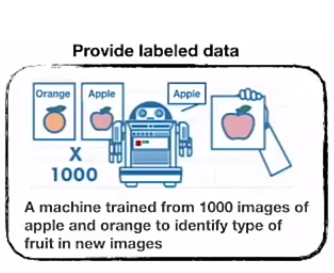
\includegraphics[width=0.48\textwidth]{figures/survey-types-learning-sup.png}}
	 \subfigure[Unsupervised learning]{\label{unsup-learn}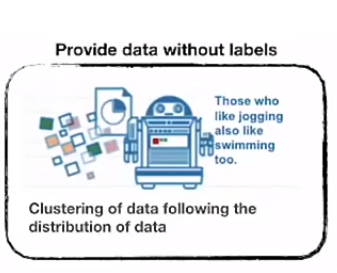
\includegraphics[width=0.48\textwidth]{figures/survey-types-learning-unsup.png}}
 	 \subfigure[Semi-supervised learning]{\label{semi-sup-learn}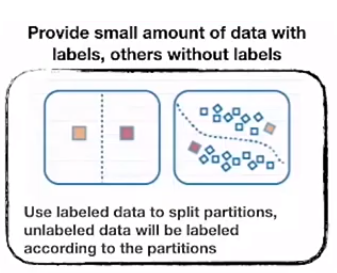
\includegraphics[width=0.48\textwidth]{figures/survey-types-learning-semi.png}}
	 \subfigure[Reinforcement learning]{\label{reinfo-learn}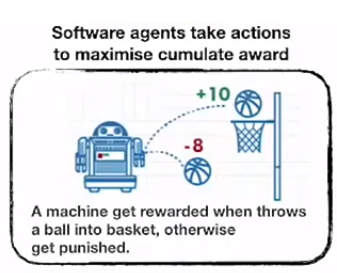
\includegraphics[width=0.48\textwidth]{figures/survey-types-learning-reinfo.png}}
	 \caption{Types of deep learning techniques}
	 \label{survey-learning-types}
\end{figure}
%

%
%----------------------------------------------------
\subsection{Survey 1}

% Author:
Abawaja

% Title: 
Identifying Malware on Cyber Physical Systems by incorporating Semi-Supervised Approach and Deep Learning

% Brief Overview:
In this research jemal et. Al. has proposed a malware detection engine that will identify malware by using semi-supervised approach with deep learning. The authors have used parallel processing to get fast results. Even though , they are using the strength of both supervised and unsupervised learning, the scheme suffers from number of shortcomings.

% Pros

% Cons

% Comparative Analysis with our work
The biggest drawback is this scheme requires a vast history of application signatures to get labelled data. It will fail when malware will constantly improve and increase its ability to blen in with the application or being undetectable by using advanced techniques. The trouble will increase with larger attack surfaces with many places to hide.

Another limitation of this approach is the use of static features which will limit the detection of runtime attacks. In cyber race , evolutions happen in milliseconds making this scheme unscalable.

%
%----------------------------------------------------
\subsection{Survey 2}

% Brief Overview:

% Pros

% Cons

% Comparative Analysis with our work


%
%----------------------------------------------------
\subsection{Survey 3}

% Brief Overview:

% Pros

% Cons

% Comparative Analysis with our work


%
%----------------------------------------------------
\subsection{Survey 3}

% Brief Overview:

% Pros

% Cons

% Comparative Analysis with our work


%
%----------------------------------------------------
\subsection{Summary of the Surveyed Research Work}



%
%==========================
\section{System Model and Evaluation Metrics}

%
%----------------------------------------------------
\subsection{Scope of the Research}

% In this section, we describe the scope and limitations of the research

%
%----------------------------------------------------
\subsection{Frequently Used Terms}

%
%----------------------------------------------------
\subsection{System Model}

% Articulate the methamatical model of the system 

%
%----------------------------------------------------
\subsection{Evaluation Metrics}

% Define terms like accuracy, error, convergence, correctness, etc.

%
%----------------------------------------------------
\subsection{Simulation Model}

% Define simulation parameteres and asumptions made

%
%----------------------------------------------------
\subsection{Simulator Design Architecture}


%
%----------------------------------------------------
\subsection{Simulation Inputs and Desired Output}


%
%==========================
\section{Proposed Protocol}

%
%----------------------------------------------------
\subsection{Describe the Protocol}

%
%----------------------------------------------------
\subsection{Present the Pseudo Code of the Protocol}

%
%----------------------------------------------------
\subsection{Describe the State Diagram of the Protocol}

%
%----------------------------------------------------
\subsection{Describe the Activity Diagram of the Protocol}


%
%----------------------------------------------------
\subsection{Critically analyze the Protocol}

% Describe the Pros, Cons and the Future work of the propsoed protocol


%
%==========================
\section{Simulation and Results}


%
%==========================
\section{Conclusion}
 
%
%==========================

%\bibliographystyle{IEEEtran}
\bibliographystyle{splncs}
\footnotesize{
%\bibliographystyle{plainnat}
%\bibliography{RP2016_MIS_v1}
}
%============================================================
%
\end{document}